\subsection{問題文}
実数値関数$u(x, t)$が$-\infty < x < \infty, t \geq 0$で定義されている.
ここで$x, t$は独立である.偏微分方程式
\begin{equation}
    \pdiff[2]{u}{t} = c^{2}\pdiff[2]{u}{x}\label{eq:subsec2:prom2}
\end{equation}
の解を初期条件
\begin{align}
    & u(x, 0) = \exp\left(-ax^{2}\right)\label{eq:subsec2:prom2_syoki1}\\
    & \pdiff{u}{t}(x, 0) = 0\label{eq:subsec2:prom2_syoki2}
\end{align}
の下で求める.但し,$a, c$は正の実数であり,$\imag$は虚数単位とする.以下の問いに答えよ.
\begin{enumerate}[(1)]
    \setlength{\itemsep}{10pt}
    \item 次の式を複素積分を用いて計算せよ.\label{subsec2:prom1}
    \begin{equation*}
        \dint{-\infty}{\infty}{\exp\left(-a(x + \imag d)^{2}\right)}
    \end{equation*}
    但し,$d$は実数である.
    また,以下の式を用いてもよい
    \begin{equation*}
        \dint{-\infty}{\infty}{\exp\left(-x^2\right)} = \sqrt{\pi}
    \end{equation*}
    \item $u(x, t)$の$x$に関するフーリエ変換$U(k, t)$を以下のように定義する.\label{subsec2:prom2}
    \begin{equation*}
        U(k, t) = \frac{1}{\sqrt{2\pi}}\dint{-\infty}{\infty}{u(x, t)\exp(-\imag kx)}
    \end{equation*}
    ここで$x$に関する積分と$t$に関する積分の順序の交換が可能であると仮定してよい.さらに,$u(x, t)$と
    $\pdiff{u}{x}(x, t)$は任意の$t$に対して$x \rightarrow\pm\infty$の時0に収束するものとする.
    \begin{enumerate}[(i)]
        \setlength{\itemsep}{10pt}
        \item $u(x, t)$が式\eqref{eq:subsec2:prom2}を満たすとき,$U(k, t)$が従う偏微分方程式を答えよ.\label{subsec2:prom2:prom1}
        \item \eqref{subsec2:prom2:prom1}の解は式\eqref{eq:subsec2:prom2_syoki2}の初期条件の下で$k$を変数とする関数$F(k)$を用いて以下のように表せることを示せ.\label{subsec2:prom2:prom2}
        \begin{equation*}
            U(k, t) = F(k)\cos(kct)
        \end{equation*}
        \item さらに式\eqref{eq:subsec2:prom2_syoki1}の初期条件の下で$F(k)$を求め,$U(k, t)$を与えよ.設問\eqref{subsec2:prom1}の結果を用いてもよい.\label{subsec2:prom2:prom3}
    \end{enumerate}
    \item 設問\ref{subsec2:prom2}で得られた$U(k, t)$のフーリエ逆変換を計算することにより,$u(x, t)$を求めよ.但し,フーリエ逆変換は次式で定義される.\label{subsec2:prom3}
    \begin{equation*}
        u(x, t) = \frac{1}{\sqrt{2\pi}}\dint[k]{-\infty}{\infty}{U(k, t)\exp(\imag kx)}
    \end{equation*}
\end{enumerate}

\newpage

\subsection{解答例}
\begin{enumerate}[(1)]
    \setlength{\itemsep}{10pt}
    \item 題意の式は複素数$f(z) = \exp(-az^2)$とおくと$R (\in \mathbb{R})$を用いて,直線$\gamma_1(t)= t + \imag d:\, t\in [-R, R]$における以下のような複素積分となる.
    \begin{align}
        & \dint{-\infty}{\infty}{\exp\left\{-a(x + \imag d)^{2}\right\}}\nonumber\\ 
        &= \lim_{R \to \infty} \dint[z]{\gamma_1}{}{\exp\left(-az^{2}\right)}\nonumber\\
        &= \lim_{R \to \infty} \dint[z]{\gamma_1}{}{f(z)}\label{eq:subsec2:prom1:hodai}
    \end{align}
    よって,式\eqref{eq:subsec2:prom1:hodai}を求めればいいことが分かるので,この式の値を以下で求める.

    ここで,以下の積分路$C:\gamma_1 + \gamma_2 + \gamma_3 + \gamma_4$を考える.
    \begin{center}
        \begin{tikzpicture}[>=stealth]
            \coordinate (O) at (0, 0);
            \draw [->] ($(O) + (-2, 0)$) -- ($(O) + (2, 0)$) node [right] {$\mathrm{Re}$};
            \draw [->] ($(O) + (0, -2)$) -- ($(O) + (0, 2)$) node [left] {$\mathrm{Im}$};
            \coordinate (LR) at (-1, 0) node at (LR) [below] {$-R$};
            \coordinate (RR) at (1, 0) node at (RR)[below] {$R$};
            \coordinate (D) at (0, 1) node at (D) [above right] {$d$};
            \coordinate (LD) at (-1, 1);
            \coordinate (RD) at (1, 1);
            \draw [very thick, ->] (LD) -- ($(LD)!0.3!(RD)$) node [above] {$\gamma_1$};
            \draw [very thick] ($(LD)!0.3!(RD)$) -- (RD);
            \draw [very thick, ->] (LR) -- ($(LR)!0.3!(LD)$) node [left] {$\gamma_2$};
            \draw [very thick] ($(LR)!0.3!(LD)$) -- (LD);
            \draw [very thick] (LR) -- ($(LR)!0.7!(RR)$) node [below] {$\gamma_3$};
            \draw [very thick, <-] ($(LR)!0.7!(RR)$) -- (RR);
            \draw [very thick] (RR) -- ($(RR)!0.7!(RD)$) node [right] {$\gamma_4$};
            \draw [very thick, <-] ($(RR)!0.7!(RD)$) -- (RD);
        \end{tikzpicture}
    \end{center}
    よって,この時,$f(z) = \exp(-az^2)$は$\mathbb{C}$上で正則であるので,積分路$C$及び$C$内で正則より,
    Cauchyの積分定理より以下が成り立つ.
    \begin{equation}
        \dint[z]{C}{}{f(z)} = 0\label{eq:subsec2:prom1:caucy}
    \end{equation}
    よって,またここで以下が成り立つ.
    \begin{equation}
        \dint[z]{C}{}{f(z)} = \dint[z]{\gamma_1}{}{f(z)} + \dint[z]{\gamma_2}{}{f(z)} + \dint[z]{\gamma_3}{}{f(z)} + \dint[z]{\gamma_4}{}{f(z)}\label{eq:subsec2:prom1:sekibun}
    \end{equation}
    従って,積分路$\gamma_1, \gamma_2, \gamma_3, \gamma_4$における積分について以下が成り立つ.
    
    % まず,$\gamma_1$の積分については求める式\eqref{eq:subsec2:prom1:hodai}である.
    % \begin{align}
    %     \dint[z]{\gamma_1}{}{f(z)} 
    %     &= \dint[t]{-R}{R}{\exp\left(-a(t + \imag d)^2\right)}\label{eq:subsec2:prom1:gamma1}
    %     % &= \dint[t]{-R}{R}{\exp\left(-a(t^2 + 2\imag dt - d^2)\right)}\nonumber\\
    %     % \mbox{オイラーの公式より}&\nonumber\\
    %     % &= \dint[t]{-R}{R}{\exp\left(-at^2 + ad^2\right)\left\{\cos(2dt) + \imag \sin(2dt)\right\}}\nonumber\\
    %     % \sin(2dt)\mbox{は奇関数より}&\nonumber\\
    %     % &= \dint[t]{-R}{R}{\exp\left(-at^2 + ad^2\right)\cos(2dt)}\label{eq:subsec2:prom1:gamma1}
    % \end{align}

    まず,$\gamma_2$の積分について$\gamma_2(t) = -R + \imag t\, : \, t\, \in \, \left[0, d\right]$より以下が成り立つ.
    \begin{align}
        \dint[z]{\gamma_2}{}{f(z)} 
        &= \dint[t]{0}{d}{\exp\left(-a(-R + \imag t)^2\right)\imag}\nonumber\\
        &= \dint[t]{0}{d}{\exp\left(-a(R^2 - 2\imag Rt - t^2)\right)\imag}\label{eq:subsec2:prom1:gamma2}
    \end{align}
    次に,$\gamma_3$の積分について$\gamma_3(t) = t\, : \, t\, \in \, \left[-R, R\right]$より以下が成り立つ.
    \begin{align}
        \dint[z]{\gamma_3}{}{f(z)} 
        &= \dint[t]{R}{-R}{\exp\left(-at^2\right)}\label{eq:subsec2:prom1:gamma3}
    \end{align}
    次に,$\gamma_4$の積分について$\gamma_4(t) = R + \imag t\, : \, t\, \in \, \left[0, d\right]$より以下が成り立つ.
    \begin{align}
        \dint[z]{\gamma_4}{}{f(z)} 
        &= \dint[t]{0}{d}{\exp\left(-a(R + \imag t)^2\right)\imag}\nonumber\\
        &= \dint[t]{0}{d}{\exp\left(-a(R^2 + 2\imag Rt - t^2)\right)\imag}\label{eq:subsec2:prom1:gamma4}
    \end{align}
    従って,式\eqref{eq:subsec2:prom1:gamma2}より,以下が成り立つ.
    \begin{align*}
        \left\lvert \dint[t]{0}{d}{\exp\left(-a(R^2 - 2\imag Rt - t^2)\right)\imag}\right\rvert
        &\leq \, \dint[t]{0}{d}{\left\lvert\exp\left(-a(R^2 - 2\imag Rt - t^2)\right)\imag\right\rvert}\\
        &= \, \dint[t]{0}{d}{\left\lvert\exp\left(-a(R^2 - 2\imag Rt - t^2)\right)\right\rvert\mid\imag\mid}\\
        &= \, \dint[t]{0}{d}{\left\lvert\exp\left(-aR^2\right)\right\rvert\left\lvert\exp\left(- 2\imag Rt\right)\right\rvert\left\lvert\exp\left(- t^2\right)\right\rvert}\\
        &= \, \dint[t]{0}{d}{\left\lvert\exp\left(-aR^2\right)\right\rvert\left\lvert\exp\left(- t^2\right)\right\rvert}\\
        &= \, \exp\left(-aR^2\right)\dint[t]{0}{d}{\exp\left(- t^2\right)}\\
        \therefore \lim_{R \to \infty} \dint[t]{0}{d}{\left\lvert\exp\left(-a(R^2 - 2\imag Rt - t^2)\right)\imag\right\rvert}
        &= \lim_{R \to \infty}\exp\left(-aR^2\right)\dint[t]{0}{d}{\exp\left(- t^2\right)} = 0
    \end{align*}
    挟み撃ちの定理より
    \begin{align}
        &\lim_{R \to \infty} \left\lvert \dint[t]{0}{d}{\exp\left(-a(R^2 - 2\imag Rt - t^2)\right)\imag}\right\rvert = 0\nonumber\\
        &\therefore\, \lim_{R \to \infty} \dint[t]{0}{d}{\exp\left(-a(R^2 - 2\imag Rt - t^2)\right)\imag} = 0\label{eq:subsec2:prom1:gamma2:kyokugen}
    \end{align}
    また,式\eqref{eq:subsec2:prom1:gamma4}より,同様にして以下が成り立つ.
    \begin{align*}
        \left\lvert \dint[t]{0}{d}{\exp\left(-a(R^2 + 2\imag Rt - t^2)\right)\imag}\right\rvert
        &\leq \, \exp\left(-aR^2\right)\dint[t]{0}{d}{\exp\left(- t^2\right)}\\
        \therefore \lim_{R \to \infty} \dint[t]{0}{d}{\left\lvert\exp\left(-a(R^2 - 2\imag Rt - t^2)\right)\imag\right\rvert}
        &= \lim_{R \to \infty}\exp\left(-aR^2\right)\dint[t]{0}{d}{\exp\left(- t^2\right)} = 0
    \end{align*}
    挟み撃ちの定理より
    \begin{align}
        &\lim_{R \to \infty} \left\lvert \dint[t]{0}{d}{\exp\left(-a(R^2 - 2\imag Rt - t^2)\right)\imag}\right\rvert = 0\nonumber\\
        &\therefore\, \lim_{R \to \infty} \dint[t]{0}{d}{\exp\left(-a(R^2 - 2\imag Rt - t^2)\right)\imag} = 0\label{eq:subsec2:prom1:gamma4:kyokugen}
    \end{align}
    また,題意の式より,以下が成り立つ.
    \begin{equation}
        \dint{-\infty}{\infty}{\exp\left(-x^2\right)} = \sqrt{\pi}\label{eq:subsec2:prom1:daii}
    \end{equation}
    また,$a > 0$より式\eqref{eq:subsec2:prom1:gamma3}から,
    $u = -\sqrt{a}t$と置換すると以下が成り立つ.
    \begin{equation}
        \dint[t]{R}{-R}{\exp\left(-at^2\right)}
        = \dint[u]{-\sqrt{a}R}{\sqrt{a}R}{\exp\left(-u^2\right)\frac{1}{-\sqrt{a}}}\label{eq:subsec2:prom1:gamma3:tikan}
    \end{equation}
    よって,式\eqref{eq:subsec2:prom1:daii}, \eqref{eq:subsec2:prom1:gamma3:tikan}より,以下のようになる.
    \begin{align}
        \lim_{R \to \infty} \dint[t]{R}{-R}{\exp\left(-at^2\right)}
        &= -\frac{1}{\sqrt{a}}\dint[u]{-\infty}{\infty}{\exp\left(-u^2\right)}\nonumber\\
        &= -\frac{\sqrt{\pi}}{\sqrt{a}}\label{eq:subsec2:prom1:gamma3:ans}
    \end{align}
    従って,式\eqref{eq:subsec2:prom1:caucy}, \eqref{eq:subsec2:prom1:gamma2:kyokugen}, 
    \eqref{eq:subsec2:prom1:gamma3:ans}, \eqref{eq:subsec2:prom1:gamma4:kyokugen}より,以下が成り立つ.
    \begin{align*}
        &\lim_{R \to \infty}\dint[z]{C}{}{f(z)} = 0\\
        \Longleftrightarrow\, &\lim_{R \to \infty} \dint[z]{\gamma_1}{}{f(z)} + \lim_{R \to \infty} \dint[z]{\gamma_2}{}{f(z)} + \lim_{R \to \infty} \dint[z]{\gamma_3}{}{f(z)}
         + \lim_{R \to \infty} \dint[z]{\gamma_4}{}{f(z)} = 0\\
        \Longleftrightarrow\, &\lim_{R \to \infty} \dint[z]{\gamma_1}{}{f(z)} + 0 + \left(-\sqrt{\frac{\pi}{a}}\right)
         + 0 = 0\\
        \Longleftrightarrow\, &\lim_{R \to \infty} \dint[z]{\gamma_1}{}{f(z)} = \sqrt{\frac{\pi}{a}}
    \end{align*}
    従って,式\eqref{eq:subsec2:prom1:hodai}より求める値は$\sqrt{\frac{\pi}{a}}$となる.\\[1cm]
    (中田解)\\
    $f(z)=\exp(-az^{2})$とする.\\
    $R(\in \mathbb{R})$を用いて, 次の積分路を考える.
    \begin{center}
        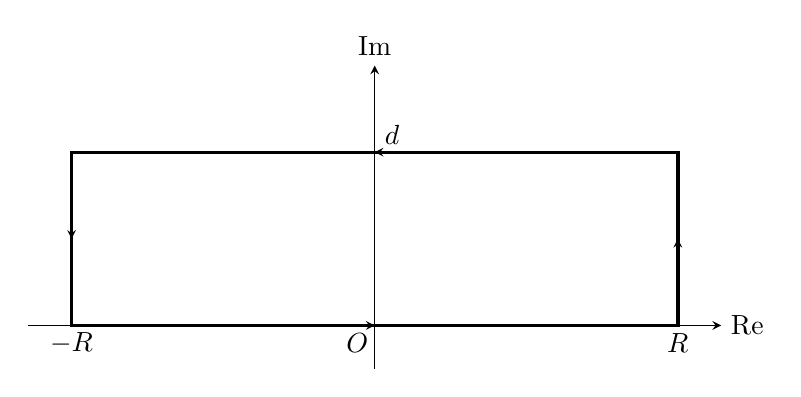
\begin{tikzpicture}[>=stealth,scale=1.1]
            \draw[->](-4,0)--(4,0) node[right] {Re};
            \draw[->](0,-0.5)--(0,3) node[above] {Im};
            \draw[very thick] (-3.5,0)--(3.5,0)--(3.5,2)--(-3.5,2)--cycle;
            \draw[->] (-0.2,0)--(0,0);
            \draw[->] (0.2,2)--(0,2);
            \draw[->] (3.5,0.8)--(3.5,1);
            \draw[->] (-3.5,1.2)--(-3.5,1);
            \node at(-3.5,-0.2) {$-R$};
            \node at(3.5,-0.2) {$R$};
            \node at(0.2,2.2) {$\imag d$};
            \node at(-0.2,-0.2) {$O$};
        \end{tikzpicture}
    \end{center}
    $e^{-az^{2}}$に留数は存在しないので, 上の周回積分路$C$において
    \begin{eqnarray*}
        \dint[z]{C}{}{\exp(-az^{2})}=0 
    \end{eqnarray*}
    ここで, $-R\to R$の積分路を$C_{1}$とし, $R\to R+\imag d$の積分路を$C_{2}$, $R+\imag d\to -R+\imag d$の積分路を$C_{3}$, $-R+\imag d\to -R$の積分路を$C_{4}$とすると,
    \begin{eqnarray*}
        C = C_{1}+C_{2}+C_{3}+C_{4}
    \end{eqnarray*}
    である. ここで,$R \to \infty$において
    \begin{eqnarray*}
        \lim_{R\to \infty}\dint[z]{C_{2}}{}{\exp(-az^{2})} 
        &=& \lim_{R\to \infty}\dint[t]{0}{d}{\exp(-a(R+\imag t)^{2})}\\
        &=&0
    \end{eqnarray*}
    同様にして
    \begin{eqnarray*}
        \lim_{R\to \infty}\dint[z]{C_{4}}{}{\exp(-az^{2})} 
        &=& \lim_{R\to \infty}\dint[t]{d}{0}{\exp(-a(-R+\imag t)^{2})}\\
        &=& 0
    \end{eqnarray*}
    となるので,
    \begin{eqnarray*}
        \lim_{R\to \infty}\dint[z]{C}{}{\exp(-az^{2})} 
        &=& \lim_{R\to \infty}\dint[z]{C_{1}}{}{\exp(-az^{2})}+\lim_{R\to \infty}\dint[z]{C_{3}}{}{\exp(-az+\imag d)}\\
        &=& 0
    \end{eqnarray*}
    したがって,
    \begin{eqnarray*}
        \dint{-\infty}{\infty}{\exp(-ax^{2})} = \dint{-\infty}{\infty}{\exp(-a(x+\imag d)^{2})}
    \end{eqnarray*}
    ここで, $t=\sqrt{a}x$とおくと,
    \begin{eqnarray*}
        \frac{{\rm d}t}{{\rm d}x}=\sqrt{a}\ \Longleftrightarrow\ {\rm d}x = \frac{1}{\sqrt{a}}\,{\rm d}t
    \end{eqnarray*}
    であるから,
    \begin{eqnarray*}
        \dint{-\infty}{\infty}{\exp(-ax^{2})} &=& \dint[t]{-\infty}{\infty}{\exp(-t^{2})\cdot \frac{1}{\sqrt{a}}}\\
                                              &=& \frac{1}{\sqrt{a}}\dint{-\infty}{\infty}{\exp(-x^{2})}\\
                                              &=& \sqrt{\frac{\pi}{a}}
    \end{eqnarray*}
    よって,
    \begin{eqnarray*}
        \dint{-\infty}{\infty}{\exp(-a(x+\imag d))} = \sqrt{\frac{\pi}{a}}
    \end{eqnarray*}
    \item 
    \begin{enumerate}[(i)]
        \setlength{\itemsep}{10pt}
        \item 式\eqref{eq:subsec2:prom2}と題意より,以下が成り立つ.
        \begin{align*}
            \pdiff[2]{U(k, t)}{t} 
            & = \pdiff[2]{\left(\frac{1}{\sqrt{2\pi}}\dint{-\infty}{\infty}{u(x, t)\exp(-\imag kx)}\right)}{t}\\
            & = \frac{1}{\sqrt{2\pi}}\dint{-\infty}{\infty}{\pdiff[2]{u(x, t)}{t}\exp(-\imag kx)}\\
            & = \frac{1}{\sqrt{2\pi}}\dint{-\infty}{\infty}{c^{2}\pdiff[2]{u(x, t)}{x}\exp(-\imag kx)}\\
            & = \frac{c^{2}}{\sqrt{2\pi}}\left\{\left[\pdiff{u(x, t)}{x}\exp(-\imag kx)\right]_{-\infty}^{\infty} - (-\imag k)\dint{-\infty}{\infty}{\pdiff{u(x, t)}{x}\exp(-\imag kx)}\right\}\\
            & = \frac{\imag kc^{2}}{\sqrt{2\pi}}\dint{-\infty}{\infty}{\pdiff{u(x, t)}{x}\exp(-\imag kx)}\\
            & = \frac{\imag kc^{2}}{\sqrt{2\pi}}\left\{\left[u(x, t)\exp(-\imag kx)\right]_{-\infty}^{\infty} - (-\imag k)\dint{-\infty}{\infty}{u(x, t)\exp(-\imag kx)}\right\}\\
            & = \frac{(\imag kc)^{2}}{\sqrt{2\pi}}\dint{-\infty}{\infty}{u(x, t)\exp(-\imag kx)}\\
            & = -(kc)^{2}U(k, t)
        \end{align*}
        よって,$U(k, t)$は以下の偏微分方程式に従う.
        \begin{equation}
            \pdiff[2]{U(k, t)}{t} = -(kc)^{2}U(k, t)\label{eq:subsec2:ans1}
        \end{equation}
        \item 初期条件\eqref{eq:subsec2:prom2_syoki2}より,以下のことが成り立つ.
        \begin{align*}
            \pdiff{U(k, t)}{t} 
            & = \pdiff{\left(\frac{1}{\sqrt{2\pi}}\dint{-\infty}{\infty}{u(x, t)\exp(-\imag kx)}\right)}{t}\\
            & = \frac{1}{\sqrt{2\pi}}\dint{-\infty}{\infty}{\pdiff{u(x, t)}{t}\exp(-\imag kx)}\\
        \end{align*}
        \begin{equation}
            \therefore\, \pdiff{U}{t}(k, 0) 
             = \frac{1}{\sqrt{2\pi}}\dint{-\infty}{\infty}{\pdiff{u}{t}(x, 0)\exp(-\imag kx)} = 0\label{eq:subsec2:ans2_ini1}
        \end{equation}
        よって,$U(k, t)$に関する初期条件も式\eqref{eq:subsec2:ans2_ini1}のようになる.ここで$U(k, t)$が題意の関数で表されるとすると
        $U(k, t)$の$t$に関する1階偏微分を行うと以下のようになる.
        \begin{align*}
            \pdiff{U(k, t)}{t} &= \pdiff{F(k)\cos(kct)}{t}\\
            &= F(k)(-kc\sin(kct))
        \end{align*}
        よって,以下が成り立つ.
        \begin{equation}
            \pdiff{U}{t}(k, 0) = F(k)(-kc\sin(kc\cdot 0)) = 0\label{eq:subsec2:ans2_ini2}
        \end{equation}
        よって,題意の関数でおくと初期条件\eqref{eq:subsec2:ans2_ini1}を満たす.
        また,\eqref{subsec2:prom2:prom1}の解となるかを以下に示す.
        
        \eqref{subsec2:prom2:prom1}の式に代入して,
        \begin{align*}
            \mbox{(左辺)}
            &= \pdiff[2]{U(k, t)}{t} \\
            &= \pdiff[2]{\left(F(k)\cos(kct)\right)}{t}\\
            &= -(kc)^{2}F(k)\cos(kct)\\
            &= -(kc)^{2}U(k, t)\\
            &= \mbox{(右辺)}
        \end{align*}
        よって,$U(k, t) = F(k)\cos(kct)$は\eqref{subsec2:prom2:prom1}の解の一つである.従って,式\eqref{eq:subsec2:prom2_syoki2}
        の初期条件のもとで\eqref{subsec2:prom2:prom1}の解となることが示されたので,題意は示された.
        \item 式\eqref{eq:subsec2:prom2_syoki1}の初期条件の下で設問\eqref{subsec2:prom1}より,以下が成り立つ.
        \begin{align*}
            U(k, 0) &= \frac{1}{\sqrt{2\pi}}\dint{-\infty}{\infty}{u(x, 0)\exp(-\imag kx)}\\ 
            &= \frac{1}{\sqrt{2\pi}}\dint{-\infty}{\infty}{\exp\left(-ax^{2}\right)\exp(-\imag kx)}\\
            &= \frac{1}{\sqrt{2\pi}}\dint{-\infty}{\infty}{\exp\left(-ax^{2}-\imag kx\right)}\\
            &= \frac{1}{\sqrt{2\pi}}\dint{-\infty}{\infty}{\exp\left\{-a\left(x - \frac{\imag k}{2a}\right)^{2} + \frac{1}{a}\cdot \left(\frac{\imag k}{2}\right)^{2}\right\}}\\
            &= \frac{\exp \left(-\frac{k^{2}}{4a}\right)}{\sqrt{2\pi}}\dint{-\infty}{\infty}{\exp\left\{-a\left(x - \frac{\imag k}{2a}\right)^{2}\right\}}\\
            &= \frac{\exp \left(-\frac{k^{2}}{4a}\right)}{\sqrt{2\pi}}\sqrt{\frac{\pi}{a}}
        \end{align*}
        従って以下が成り立つ.
        \begin{align*}
            U(k, 0) = F(k)\cos(kc\cdot 0) = F(k) = \frac{\exp \left(-\frac{k^{2}}{4a}\right)}{\sqrt{2a}}
        \end{align*}
        よって,$U(k, t)$は以下のようになる
        \begin{equation}
            U(k, t) = F(k)\cos(kct) = \frac{\exp \left(-\frac{k^{2}}{4a}\right)}{\sqrt{2a}}\cos(kct)
        \end{equation}
    \end{enumerate}
  \item 設問\eqref{subsec2:prom2}で得られた$U(k, t)$と$a > 0$, 設問\eqref{subsec2:prom1}より,以下が成り立つ.
    \begin{align*}
        u(x, t) &= \frac{1}{\sqrt{2\pi}}\dint[k]{-\infty}{\infty}{U(k, t)\exp(ikx)}\\
        &= \frac{1}{\sqrt{2\pi}}\dint[k]{-\infty}{\infty}{\frac{\exp\left(\frac{-k^2}{4a}\right)}{\sqrt{2a}}\cos(kct)\exp(\imag kx)}\\
        &= \frac{1}{2\sqrt{a\pi}}\dint[k]{-\infty}{\infty}{\exp\left(-\frac{k^2}{4a} + \imag kx\right)\frac{\exp\left(\imag kct\right) + \exp\left(-\imag kct\right)}{2}}\\
        &= \frac{1}{4\sqrt{a\pi}}\dint[k]{-\infty}{\infty}{\exp\left(-\frac{k^2}{4a} + \imag kx + \imag kct\right) + \exp\left(-\frac{k^2}{4a} + \imag kx - \imag kct\right)}\\
        &= \frac{1}{4\sqrt{a\pi}}\dint[k]{-\infty}{\infty}{\exp\left[-\frac{1}{4a}\left\{k - 2a\imag (x + ct)\right\}^2 - a(x + ct)^2\right]}\\
        &\quad+ \frac{1}{4\sqrt{a\pi}}\dint[k]{-\infty}{\infty}{\exp\left[-\frac{1}{4a}\left\{k - 2a\imag (x - ct)\right\}^2 - a(x - ct)^2\right]}\\
        &= \frac{1}{4\sqrt{a\pi}}\exp\left\{-a(x + ct)^2\right\}\dint[k]{-\infty}{\infty}{\exp\left[-\frac{1}{4a}\left\{k - 2a\imag (x + ct\right\}^2\right]}\\
        &\quad+ \frac{1}{4\sqrt{a\pi}}\exp\left\{-a(x - ct)^2\right\}\dint[k]{-\infty}{\infty}{\exp\left[-\frac{1}{4a}\left\{k - 2a\imag (x - ct)\right\}^2\right]}\\
        &= \frac{1}{4\sqrt{a\pi}}\exp\left\{-a(x + ct)^2\right\}\sqrt{\frac{\pi}{\frac{1}{4a}}} + \frac{1}{4\sqrt{a\pi}}\exp\left\{-a(x - ct)^2\right\}\sqrt{\frac{\pi}{\frac{1}{4a}}}\\
        &= \frac{1}{2}\left[\exp\left\{-a(x + ct)^2\right\} + \exp\left\{-a(x - ct)^2\right\}\right]
     \end{align*}
    よって,求める関数$u(x, t)$は以下のようになる.
    \begin{equation*}
        u(x, t) = \frac{1}{2}\left[\exp\left\{-a(x + ct)^2\right\} + \exp\left\{-a(x - ct)^2\right\}\right]
    \end{equation*}
\end{enumerate}